% ============================================================================
% Spatial Context Causal Adjustment for Geographic Observational Studies
% ============================================================================
% Target journal: International Journal of Geographical Information Science
% ============================================================================
\documentclass{article}

\usepackage{amsmath,amssymb}
\usepackage{booktabs}
\usepackage{graphicx}
\usepackage{array}
\usepackage{caption}
\usepackage{hyperref}
\usepackage{natbib}
\usepackage{tikz}
\usetikzlibrary{positioning,arrows.meta,shapes.geometric,fit,calc}
\graphicspath{{./figures/}{./}}
\bibliographystyle{plainnat}
\setlength{\emergencystretch}{2em}
\newenvironment{keywords}{\par\noindent\textbf{Keywords:}\ }{\par}
\newcommand{\ruleversion}{the 2026-06-30 evidence-grade rule set}
\newcolumntype{L}[1]{>{\raggedright\arraybackslash}p{#1}}

\begin{document}

\title{\parbox{0.9\textwidth}{\centering Spatial Context Causal Adjustment:\\A Diagnostic Workflow for Geographic Observational Studies}}

\author{Author information removed for double-anonymous review}

\date{}
\maketitle

\begin{abstract}
Geographic observational studies often combine spatially structured treatments, outcomes, and environmental context. Standard causal estimators can be used in these studies, but their credibility depends on whether spatial context is a defensible adjustment source and on whether residual spatial structure is reported rather than hidden.

We introduce Spatial Context Causal Adjustment (SCCA), a diagnostic audit workflow for spatial-context adjustment sets. SCCA is not a new identification theorem. It standardises context construction, adjustment-set comparison, support, balance, spatial bootstrap, threshold placebos, residual spatial autocorrelation, graph sensitivity, variable-role audits, residual spatial bias-bound reporting where graph inputs exist, and rule-based evidence grades. Residual Moran's $I$ and the bias-bound diagnostic are warning boundaries, not identifying statistics. The default residual-Moran material threshold is calibrated in a 2{,}880-fit controlled design spanning SAR, CAR, distance-kernel, and non-stationary latent spatial processes.

We evaluate SCCA with synthetic stress tests, a Chongqing urban heat case, a county GIS reproducibility check, and a synthetic positive control. In Chongqing, the treatment is building-level high-rise status but the outcome is MODIS summer LST on a $\sim$1\,km grid. The primary empirical quantity is therefore an outcome-scale pixel model: the slope relating pixel-mean high-rise share to pixel-mean LST was 0.546$^\circ$C per unit share (95\% CI [0.359, 0.734]), not a building-level ATT. The building-level matching ATT was 0.303$^\circ$C (95\% CI [0.220, 0.383]) and is retained only as a diagnostic approximation. Clustering on the shared outcome pixel widened the building-level OLS standard error by 41.5\%. The preferred pre-treatment matching design slightly missed the strict balance rule (maximum post-match SMD = 0.104), and the matched residual Moran's $I = 0.112$ ($p=0.01$) crossed the default 0.10 material threshold by 0.012. The grade is therefore bounded support under the default rule and remains a residual-spatial warning under higher thresholds. The calibration also shows that this warning is process-dependent: at $t=0.10$, true-positive rates are 0.194 for CAR, 0.529 for SAR, 0.994 for distance-kernel, and 1.000 for non-stationary latent fields. The county dataset provides ArcGIS Causal Inference algorithm comparison and spatial diagnostics rather than substantive validation; a synthetic positive control is graded core support.

SCCA contributes a reproducible protocol for auditing evidence in geographic causal analysis. It does not remove unmeasured spatial confounding, solve interference, or make restricted data fully reproducible; it makes adjustment choices, spatial diagnostics, and claim boundaries inspectable across GIS-facing workflows.
\end{abstract}

\begin{keywords}
spatial causal inference; spatial confounding; causal adjustment; evidence grading; modifiable areal unit problem; open reproducibility
\end{keywords}


% ============================================================================
\section{Introduction}
\label{sec:intro}
% ============================================================================

Geographic information science increasingly supports causal policy questions: whether urban form changes heat exposure, whether infrastructure changes disease risk, or whether land-use interventions change environmental outcomes. These questions are usually studied from observational spatial data, where treatment is rarely randomized, units are embedded in environmental gradients, and outcomes may be measured at resolutions that differ from the intervention units.

The main challenge is how to use spatial context, not whether causal estimators exist. GIS researchers already use matching, weighting, regression adjustment, difference-in-differences, spatial panels, and machine-learning estimators \citep{stuart2010matching, angrist2009mostly, athey2019estimating, hernan2020whatif}. Elevation, land cover, access, morphology, settlement history, and administrative structure can confound geographic effects; indiscriminate adjustment can also reduce support or include invalid post-treatment variables \citep{reich2021review,gilbert2021spatialconfounding,hodges2010adding,paciorek2010importance,dupont2022spatial+,khan2022restricted}.

Modern GIS workflows intensify this problem because remote-sensing, terrain, geometry, and neighborhood descriptors are easy to extract at scale \citep{anselin2014modern,brunsdon2016quantitative}. Spatial smooths or fixed effects can also corrupt treatment coefficients when treatment is spatially patterned \citep{hodges2010adding,dupont2022spatial+,tec2023spatialdml}. Geographic causal analysis therefore needs visible diagnostics for which context variables help and where the evidence stops.

This paper proposes Spatial Context Causal Adjustment (SCCA), a workflow rather than a new estimator or identification theorem. SCCA wraps standard estimators with context construction, adjustment-set comparison, support and balance diagnostics, spatial robustness tests, and an evidence grade. Its premise is conservative: context supports causal adjustment only when it improves a diagnosed design.

Our contributions are:

\begin{enumerate}
\item A formal SCCA workflow for selecting and diagnosing spatial-context adjustment sets, positioned as an audit protocol rather than a universal estimator.
\item A scale-aware claim boundary that reports outcome-support estimands when treatment and outcome are measured on different spatial supports, with building-level contrasts retained only as diagnostics in such cases.
\item A residual-spatial warning layer combining calibrated residual Moran's $I$, graph sensitivity, neighborhood exposure checks, and a conservative residual spatial bias-bound diagnostic.
\item A reproducible evidence protocol covering field-level provenance, support, balance, spatial bootstrap, threshold placebos, variable-role auditing, change-of-support diagnostics, GIS-facing outputs, and evidence grading.
\item Focused evidence from synthetic stress tests, a Chongqing urban heat case, a county ArcGIS Causal Inference parity benchmark, and a synthetic positive control certified as core support.
\end{enumerate}

Chongqing is the main case because author-controlled spatial processing links candidate context variables directly to the adjustment design. The county case is more open but uses third-party training/demo data, so it is used for ArcGIS SCI-style packaging, spatial downgrading, and interface reproducibility rather than for the main causal claim.

The paper makes a bounded claim. SCCA does not eliminate unobserved spatial confounding, solve spatial interference, or prove that richer adjustment is always better. It makes such claims harder to make without diagnostic evidence.


% ============================================================================
\section{Related Work}
\label{sec:related}
% ============================================================================

\subsection{Causal inference with spatial data}

Potential-outcome causal inference compares outcomes under treatment and control states \citep{imbens2015causal,hernan2020whatif}. Observational designs require conditional exchangeability, often operationalised by matching or weighting \citep{rosenbaum1983central, stuart2010matching}. Spatial studies make this difficult because location and environment are structured confounders. Directed acyclic graphs help separate confounders, mediators, colliders and post-treatment descendants \citep{pearl2009causality,vanderweele2015explanation}; we use this framing for candidate spatial context (Figure~\ref{fig:scca_dag}).

Spatial econometrics and spatial statistics provide tools for autocorrelation, spillover, and dependence \citep{anselin1988spatial,lesage2009introduction,anselin2014modern}. Spatial causal inference has addressed unmeasured spatial confounding, interference, and neighborhood exposure \citep{reich2021review,gilbert2021spatialconfounding,giffin2023gpsinterference,papadogeorgou2022causal,schnell2020mitigating}. A key warning is that adding spatial smooths or fixed effects can bias a spatially patterned treatment coefficient \citep{hodges2010adding,paciorek2010importance,dupont2022spatial+,khan2022restricted}; spatial double-machine-learning work similarly requires geographic cross-fitting blocks \citep{tec2023spatialdml}. These tools do not by themselves select valid adjustment sets for routine GIS workflows. SCCA therefore treats spatial-dependence diagnostics and causal-adjustment diagnostics as related but distinct.

\subsection{Spatial context as an adjustment source}

Geographic adjustment sets often include coordinates, fixed effects, distance, terrain, land cover, built environment, and remote-sensing indices. These variables can proxy for unmeasured context, but only under assumptions about timing, causal role, and compatible spatial scale \citep{gilbert2021spatialconfounding,vanderweele2015explanation}. They can also be collinear, weakly related to treatment, scale-mismatched, or post-treatment. Because scale and aggregation interact with MAUP and edge effects \citep{openshaw1984maup,fotheringham1991modifiable,manley2006maup}, SCCA requires support and balance checks before context supports a causal statement, and reports graph and threshold sensitivity.

\subsection{Continuous exposure, spatial interference, and diagnostics}

Many GIS applications use continuous or ordered exposures. Generalised propensity-score methods estimate dose-response functions \citep{hirano2004gps,zhao2020nonbinary}. Spatial settings also raise interference concerns because nearby exposure can affect outcomes. Formal spatial-interference methods address this in specialised designs \citep{verbitskysavitz2012,aronow2017interference,forastiere2021interference,giffin2023gpsinterference,papadogeorgou2022causal}. SCCA does not identify spillovers in that sense; it reports neighborhood-exposure and spatial-lag outputs as stability diagnostics.

\subsection{Diagnostics and evidence grades}

Causal estimates are often reported as single numbers even when the adjustment design is fragile. SCCA instead interprets effects together with balance, matched counts, support attrition, bootstrap stability, placebo checks, residual autocorrelation, neighbor-exposure sensitivity, and graph-specification sensitivity. The evidence grade is not a significance label; it records whether the declared rule table gives core or bounded support.

\subsection{Position relative to adjacent workflows}

SCCA is an audit layer connecting causal adjustment diagnostics with GIS-facing spatial diagnostics. It reuses standard matching, weighting, regression, GPS and SLX-style sensitivity models, but adds a shared request schema, context variants, support and balance checks, residual-spatial downgrades, and portable GIS outputs. Relative to spatial-confounding work \citep{hodges2010adding,paciorek2010importance,dupont2022spatial+,khan2022restricted,gilbert2021spatialconfounding,tec2023spatialdml}, the increment is operational: select specifications by declared causal role and carry scale, support, and residual-spatial diagnostics into one evidence contract. This audit layer is consistent with reusable computational geography \citep{nuest2021reproducible,konkol2019computational,brunsdon2016quantitative}.


% ============================================================================
\section{Spatial Context Causal Adjustment}
\label{sec:method}
% ============================================================================

\subsection{Problem formulation}

Let $i = 1,\ldots,n$ index geographic units with geometry $g_i$, treatment or exposure $T_i$, outcome $Y_i$, observed non-spatial covariates $X_i$, and candidate spatial-context variables $C_i$. The context vector may contain coordinates, geometry, terrain, land cover, remote-sensing bands or indices, and neighborhood summaries. Figure~\ref{fig:scca_dag} represents the Chongqing case: observed terrain and historical land use are candidate confounders, latent $U$ is unmeasured spatial structure, and NDVI is shown as a possible mediator requiring a role decision.

\begin{figure}[htbp]
\centering
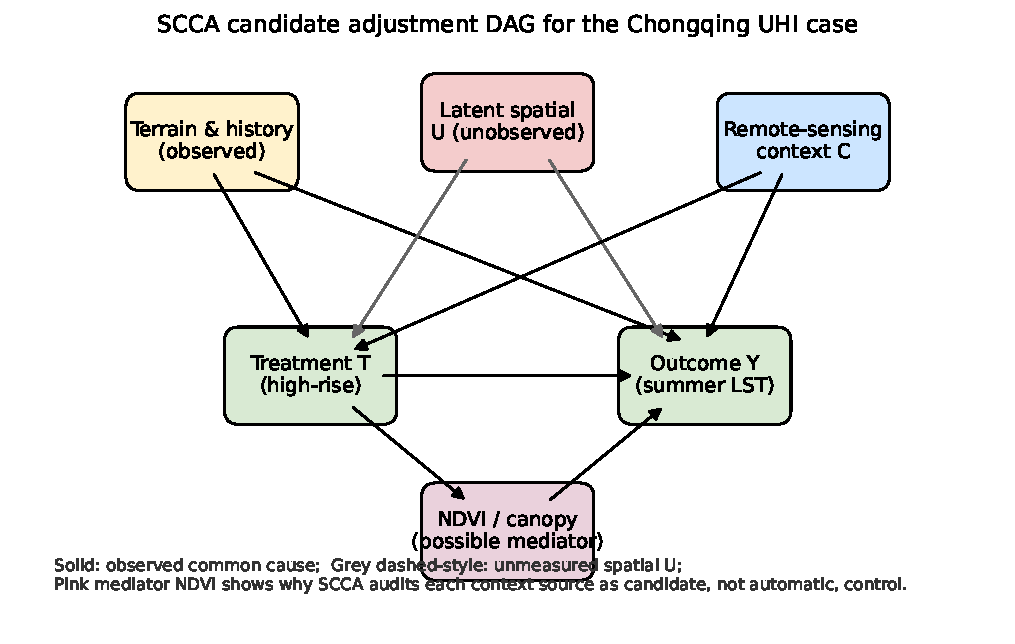
\includegraphics[width=0.9\textwidth]{fig_scca_dag.pdf}
\caption{Candidate adjustment DAG for the Chongqing UHI case. Terrain and historical land-use are observed common causes of treatment $T$ (high-rise) and outcome $Y$ (summer LST). A latent spatial process $U$ remains unobserved; SCCA reports residual Moran's $I$ and spatial-lag sensitivity as diagnostics for the resulting bias rather than identifying $U$. NDVI is shown explicitly as a possible post-treatment mediator: SCCA's variable-role layer requires the analyst to declare whether it is added as confounder or omitted as descendant of $T$.}
\label{fig:scca_dag}
\end{figure}

For binary treatment, the target estimand in the main case study is the average treatment effect on the treated:
\begin{equation}
\tau_{\mathrm{ATT}} = E[Y_i(1) - Y_i(0) \mid T_i = 1].
\end{equation}
This estimand is meaningful when treatment and outcome share a unit. When the outcome support is coarser, SCCA reports an outcome-scale estimand. In Chongqing, buildings are aggregated to MODIS LST pixels $p$, with pixel-mean high-rise share $\bar{T}_p$ and pixel-mean LST $\bar{Y}_p$. The primary coefficient is
\begin{equation}
\beta_{\mathrm{pixel}} =
\frac{\partial E[\bar{Y}_p \mid \bar{T}_p, \bar{X}_p, \bar{C}_p]}
{\partial \bar{T}_p},
\end{equation}
estimated by an adjusted pixel-level outcome model. It is a high-rise-share slope at the outcome support, not a building-level ATT. Other continuous exposures use exposure-response functions or local slopes with the same diagnostics.

SCCA does not identify $\tau_{\mathrm{ATT}}$ or $\beta_{\mathrm{pixel}}$ by itself. Identification still requires measured confounders, overlap, and limited or modeled interference. SCCA tests whether a chosen context set can support a bounded causal interpretation.

\subsection{Identification assumptions and scope}

The workflow rests on standard observational-causal assumptions stated for spatial data \citep{imbens2015causal,pearl2009causality}. Consistency requires exposure, outcome, and spatial unit to match the intervention. Conditional exchangeability requires observed covariates and context to contain relevant common causes; coordinates and remote-sensing variables are proxies, not guarantees \citep{gilbert2021spatialconfounding}. Positivity requires overlap, and no-interference and scale compatibility must be plausible or bounded. SCCA labels claim strength under these assumptions.

\subsection{Workflow}

Figure~\ref{fig:scca_workflow} summarizes the workflow: construct candidate context features, define adjustment variants, estimate the appropriate treatment or outcome model, diagnose support and balance, then run robustness checks and assign an evidence grade.

\begin{figure}[htbp]
\centering
\resizebox{0.94\textwidth}{!}{%
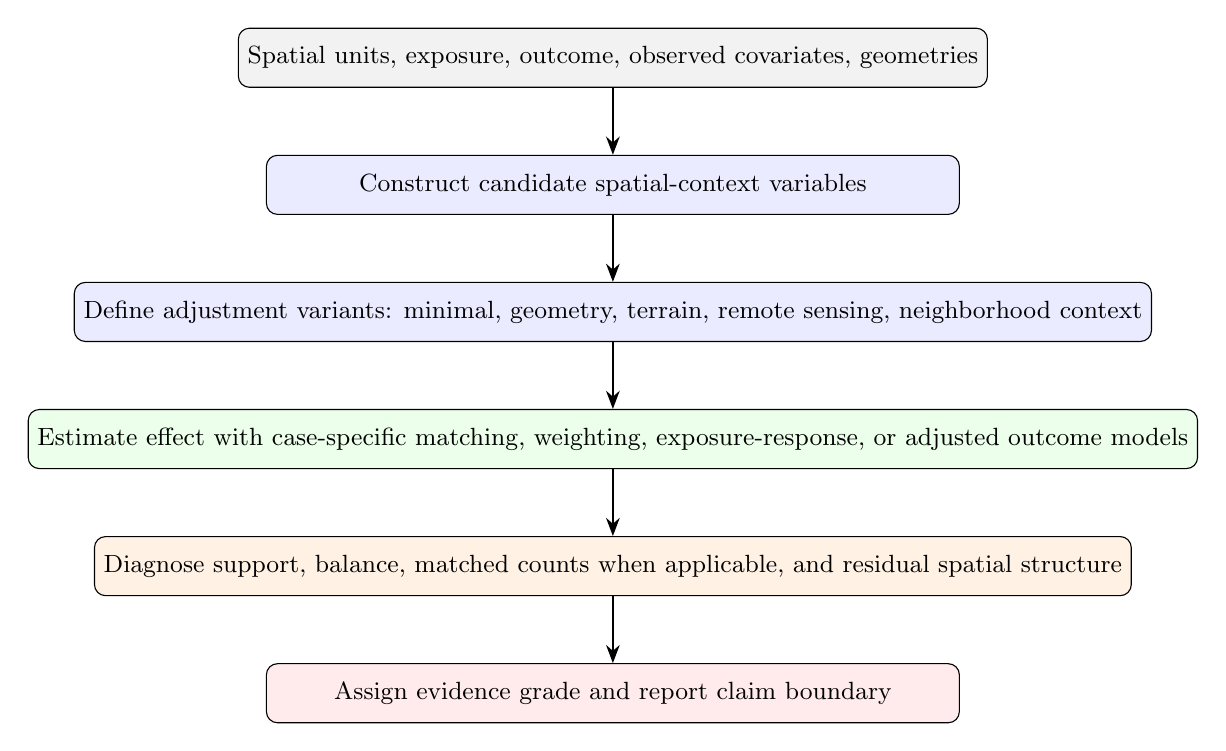
\begin{tikzpicture}[
    node distance=0.85cm,
    box/.style={draw, rounded corners, minimum height=0.75cm, minimum width=8.8cm, align=center, font=\small},
    arr/.style={-{Stealth[length=2.3mm]}, thick}
]
\node[box, fill=gray!10] (input) {Spatial units, exposure, outcome, observed covariates, geometries};
\node[box, fill=blue!8, below=of input] (context) {Construct candidate spatial-context variables};
\node[box, fill=blue!8, below=of context] (variants) {Define adjustment variants: minimal, geometry, terrain, remote sensing, neighborhood context};
\node[box, fill=green!8, below=of variants] (estimate) {Estimate effect with case-specific matching, weighting, exposure-response, or adjusted outcome models};
\node[box, fill=orange!10, below=of estimate] (diagnose) {Diagnose support, balance, matched counts when applicable, and residual spatial structure};
\node[box, fill=red!8, below=of diagnose] (grade) {Assign evidence grade and report claim boundary};
\draw[arr] (input) -- (context);
\draw[arr] (context) -- (variants);
\draw[arr] (variants) -- (estimate);
\draw[arr] (estimate) -- (diagnose);
\draw[arr] (diagnose) -- (grade);
\end{tikzpicture}
}
\caption{SCCA workflow. Spatial context is treated as a candidate adjustment source and must pass support, balance, and robustness diagnostics before it is used to support a causal claim.}
\label{fig:scca_workflow}
\end{figure}

The estimators are deliberately standard. The contribution is the diagnosable adjustment workflow and portable evidence contract.


\subsection{Adjustment variants}

SCCA does not impose one estimator on all exposure types. The reusable core estimates adjusted outcome models and ERFs for continuous or ordered exposures using generalized propensity-score weights \citep{hirano2004gps,zhao2020nonbinary}. Case modules can add binary-treatment estimators. In Chongqing, the binary module estimates
\begin{equation}
e_i = P(T_i = 1 \mid X_i, C_i)
\end{equation}
for each adjustment variant. Units outside overlap are removed, treated units are nearest-neighbor matched within caliper, and standardized mean differences (SMDs) are computed:
\begin{equation}
\mathrm{SMD}_k =
\frac{\bar{Z}_{k,T=1} - \bar{Z}_{k,T=0}}
{\sqrt{(s^2_{k,T=1} + s^2_{k,T=0})/2}},
\end{equation}
where $Z_k$ is the $k$th covariate. A variant is credible only if the maximum post-match absolute SMD is below 0.1 unless justified, and estimates are reported with matched counts and support attrition.

For continuous exposures, SCCA reports adjusted OLS, difference-outcome OLS when a baseline outcome exists, and a GPS-weighted exposure-response function. Model-based intervals describe fitted-outcome uncertainty; the evidence grade also uses spatial bootstrap, placebo, support, and residual-spatial diagnostics.

\subsection{Robustness diagnostics}

When data permit, SCCA runs spatial block bootstrap, placebo exposure definitions, weaker-outcome or placebo-outcome checks, and residual spatial autocorrelation diagnostics.

For spatial datasets, SCCA builds a neighborhood graph from polygon adjacency or coordinate $k$-nearest neighbors. The graph supports Moran diagnostics, neighbor-exposure adjustment, graph sensitivity, and an SLX-style sensitivity model \citep{lesage2009introduction}:
\begin{equation}
Y_i = \alpha + \beta T_i + \theta (WT)_i + \gamma X_i + \phi C_i + \eta (WX)_i + \lambda (WC)_i + \varepsilon_i,
\qquad \varepsilon \sim \mathcal{N}(0, \sigma^2 I),
\end{equation}
where $W$ is row-standardised. We interpret $\beta$ as the local adjusted association and $\theta$ as a neighboring-exposure signal. This is a stability diagnostic, not a full interference design.

\subsection{Diagnostic interpretation of residual Moran's I}
\label{sec:residual_diagnostic}

The residual-Moran rule is a warning boundary, not an identification result. Consider
\begin{equation}
Y_i = \tau T_i + X_i^\top \gamma + C_i^\top \phi + \sigma_u U_i + \nu_i,
\end{equation}
where $U = (I - \rho W)^{-1}\epsilon$ is a stationary SAR$(\rho)$ field and $\nu_i$ is i.i.d.\ noise. If SCCA adjusts for $(X,C)$ but not $U$, the fitted residual can be written heuristically as
\begin{equation}
r \approx M\nu + \sigma_u M U,
\end{equation}
where $M$ removes the fitted adjustment design. Residual Moran's $I$ can therefore increase when omitted spatial structure remains, but it does not identify $\rho$, $\sigma_u$, or treatment bias, and a non-significant value does not rule out spatial confounding.

SCCA therefore asks a narrower question: after the declared adjustment set is fitted, is residual spatial structure large enough to make a stronger causal statement unsafe under the rule table? Sections~\ref{sec:thresholdcalibration} and \ref{sec:chongqing_threshold_check} make this threshold auditable while keeping it diagnostic.

\subsection{Residual spatial bias-bound diagnostic}

The software layer also reports a conservative residual spatial bias-bound when a graph basis and treatment-residual vector are available. Let $R_T$ be the treatment residual after adjustment for declared covariates and admissible context, and let $\Phi_k$ contain the first $k$ non-constant low-frequency eigenvectors of the graph Laplacian. Define $P_k = \Phi_k(\Phi_k^\top\Phi_k)^{-1}\Phi_k^\top$. SCCA reports
\begin{equation}
B_{\mathrm{spatial}} =
\left(\frac{\|P_k R_T\|_2}{\|R_T\|_2}\right)
\sigma_{Y\mid X,C}\kappa_U,
\end{equation}
where $\sigma_{Y\mid X,C}$ is residual outcome variation and $\kappa_U$ is a user-declared latent smoothness scale. A graph-orthogonalization sensitivity can remove $P_kR_T$, but the bound is computed before that removal. This warning score is not an identification theorem. Small values indicate little low-frequency graph alignment; large values warn that an exposure-response result may remain aligned with graph-smooth latent structure.

\subsection{Evidence grades and threshold calibration}

SCCA assigns evidence grades with a machine-readable rule file. \textit{Core support} requires strong credibility, robust support, and no material spatial downgrade. \textit{Bounded support} marks useful evidence with explicit support, scale, balance, robustness, residual-spatial, or reproducibility limits.

The manuscript uses \ruleversion. Downgrades are triggered by moderate or weak credibility, weak support or robustness, large exposure-balance or boundary diagnostics, material residual Moran's $I$, significant neighbor exposure, large spatial-adjustment shifts, or graph-sensitivity sign changes. The default residual-Moran threshold is $t_{\mathrm{Moran}}=0.10$; the full rule table is provided in the reproduction package.

These thresholds are audit rules, not validity constants. The SMD threshold $0.10$ follows matching practice \citep{stuart2010matching,austin2009smd}; other non-Moran cutoffs remain conservative defaults. Only the residual-Moran threshold is calibrated here by sweeping spatial-process family, $\rho$, $n$ and $\sigma_u/\sigma_\nu$. The default 0.10 is a low-false-positive warning boundary; 0.20 is a high-specificity check.

A downgrade does not prove bias, and its absence does not prove identification. It only records whether a declared warning boundary was crossed. Statistically significant but sub-threshold residual Moran's $I$ is also recorded in the threshold-sensitivity table.

\subsection{Implementation surfaces}

SCCA is implemented as a shared Python core with CLI, notebook, ArcGIS Pro, and QGIS Processing adapters. The reusable \texttt{AnalysisRequest} records inputs, fields, covariates, context columns, coordinates, bootstrap groups, placebo settings, trimming thresholds, target outcomes, and \emph{variable-role} declarations. Runs write CSV, JSON, Markdown diagnostics and, for spatial inputs, common GIS outputs and QGIS \texttt{.qml} styles. For the ArcGIS comparison, the SCI Plus runner writes a machine-readable report and implements the documented continuous-exposure Causal Inference mode: regression propensity scores, matching balance, 1\%--99\% exposure trimming, and a weighted-kernel exposure-response function \citep{esri2026causalworks,wu2022matching,fan1996local}. It also writes field-level provenance and causal-risk outputs. Untested ArcGIS modes such as gradient boosting, weighting, cross-validated bandwidths, and bootstrap intervals are not claimed bit-for-bit.

The binary Chongqing module separately writes ablation, balance, matched-count, change-of-support, and matching-sensitivity tables. These outputs distinguish the outcome-scale pixel estimand from building-level matching diagnostics.

\subsection{Missing data, scale, and uncertainty}
\label{sec:missing_scale_ci}

Three conservative choices are recorded explicitly. Missing context values use within-variant median imputation with a missingness indicator added to $X$; spatially structured missingness should also trigger complete-case sensitivity. Scale and MAUP \citep{openshaw1984maup,fotheringham1991modifiable,manley2006maup} enter through the treatment unit, context resolution, and diagnostic graph. When the outcome is coarser than treatment, SCCA treats the outcome-scale coefficient as primary. In Chongqing, this is $\beta_{\mathrm{pixel}}$, the pixel-level slope relating mean high-rise share to mean LST; building-level ATT and clustered OLS remain diagnostics. SCCA also reports graph-sensitivity across $k \in \{4, 6, 8, 12\}$ and threshold-placebo sensitivity, but it does not solve scale mismatch. Uncertainty intervals come from HC3 or clustered standard errors, spatial block bootstrap quantiles, or Abadie--Imbens matching standard errors \citep{abadie2006matchingse}, as indicated in each table.


% ============================================================================
\section{Experiments}
\label{sec:experiments}
% ============================================================================

\subsection{Dataset roles and case selection}

The experiments assign different evidentiary roles to the datasets. Chongqing is the main real-data SCCA case because its high-rise treatment, geometry, terrain, remote-sensing context, and summer LST outcome are tightly coupled. It tests whether richer spatial context can support adjustment without overstating the association.

The county social-capital data instead test ArcGIS Spatial Causal Inference (SCI)-style rerun counts, output contracts, ERF/target parity, residual spatial diagnostics, and downgrading behavior for a familiar GIS example. The reproducibility scope differs by dataset (Table~\ref{tab:reproducibility_scope}); raw building-level Chongqing inputs are not redistributed.

\begin{table}[htbp]
\centering
\scriptsize
\caption{Reproducibility scope of the experimental cases.}
\label{tab:reproducibility_scope}
\resizebox{\textwidth}{!}{%
\begin{tabular}{L{3.1cm}L{3.0cm}L{4.2cm}L{4.7cm}}
\toprule
Case & Public rerun level & Restricted or source-governed inputs & Manuscript use \\
\midrule
Synthetic benchmark audit & Exact public rerun from committed generators and scripts & None beyond software dependencies & Stress-test estimator behavior under known targets \\
Chongqing urban heat & Structural rerun from public scripts, manifests, and generated summaries & Building footprints, precise coordinates, floor attributes, and derived local environmental variables require approved local access & Main real-data SCCA ablation and claim-boundary example \\
County social capital GIS run & Exact rerun where users have the licensed third-party example dataset; public outputs and scripts document the contract & Esri training/demo data and source terms govern redistribution and use & ArcGIS SCI-style trim/ERF/target parity, cross-interface output, and spatial-diagnostic downgrade check \\
\bottomrule
\end{tabular}
}
\end{table}

\subsection{Evidence synthesis design}

The experiments have four components: a synthetic benchmark across six estimator families; the Chongqing urban heat case; a county social-capital notebook/GIS run for ArcGIS SCI-style parity and portability; and a synthetic positive control that a clean design should certify as core support. Together they test the grade engine on controlled generators, real remote-sensing data, external GIS demo data, and a certified-clean design.

Table~\ref{tab:evidence_synthesis} summarizes the evidence matrix. The source table and residual-spatial threshold sensitivity outputs are included in the reproduction package.

\begin{table}[htbp]
\centering
\scriptsize
\setlength{\tabcolsep}{2pt}
\caption{SCCA evidence synthesis. Grades describe claim strength, not statistical significance alone.}
\label{tab:evidence_synthesis}
\resizebox{\textwidth}{!}{%
\begin{tabular}{L{2.2cm}L{2.0cm}L{4.0cm}L{1.7cm}L{3.2cm}}
\toprule
Case & Data type & Key diagnostic & Grade & Manuscript use \\
\midrule
Synthetic benchmark audit & Controlled generators & 48 benchmark rows; 13 robust and 29 fragile rows & Bounded support & Estimator stress test, not real-world validation \\
Chongqing urban heat & Real building and remote-sensing data & Pixel-level high-rise-share slope = 0.546$^\circ$C (primary); building-level diagnostic ATT = 0.303$^\circ$C; residual Moran's $I$ = 0.112 & Bounded support & Main real-data SCCA case with change-of-support and residual-spatial caution \\
County social capital SCI Plus run & ArcGIS algorithm reproducibility case & 3{,}044 trimmed rows; ArcGIS-mode 25 bins, scale 0.8, bandwidth 2.439; ERF MAE vs arcpy = 0.015 years; residual Moran's $I$ = 0.313 & Bounded support & Tested ArcGIS Causal Inference-mode parity plus causal-risk boundary check \\
Synthetic core-support control & Clean controlled DGP (all confounders measured) & $\widehat{\mathrm{ATT}}$ = 0.505 (true 0.5); residual Moran's $I \approx 0$ (n.s.); no downgrade rule fires & Core support & Positive control showing the core/bounded distinction is discriminative \\
\bottomrule
\end{tabular}
}
\end{table}

\subsection{Synthetic benchmark audit}

The controlled benchmark used six estimator families: matching, DiD, ERF, causal forests, spatial Granger tests, and GCCM. These 48 rows are stress tests, not empirical claims. DiD and causal forests recovered baseline targets, ERF was useful but sometimes biased, and severe-stress settings were fragile. The benchmark supports SCCA as a diagnostic wrapper, not a guarantee that every estimator works in every spatial setting.

\subsection{Chongqing urban heat case}

The main case asked whether Chongqing high-rise concentration was associated with summer land surface temperature after spatial-context adjustment. The stratified 2021 sample contained 5{,}000 buildings; treatment was at least 10 floors. MODIS MOD11A2 summer LST (June--August 2021) was sampled on its native $\sim$1\,km grid. Context variables included coordinates, footprint area, Sentinel-2 bands and indices, 30\,m SRTM elevation, and slope. Because the outcome is coarser than treatment, the primary quantity is the pixel high-rise-share slope; building-level matching is diagnostic.

\paragraph{Outcome-scale estimate and diagnostic matching.}
At the outcome resolution, the pre-treatment model estimated a 0.546$^\circ$C slope (95\% CI [0.359, 0.734]) per unit increase in pixel-mean high-rise share (Table~\ref{tab:cos}). This aligns with the MODIS support and is not a building-level ATT. The building-level matching estimate was 0.303$^\circ$C (95\% CI [0.220, 0.383]; Table~\ref{tab:chongqing}). Clustering adjusted building-level OLS on the shared outcome pixel widened the standard error from 0.038 to 0.054 (41.5\%).

\paragraph{Change of support.}
The 5{,}000 buildings map to about 1{,}400 outcome pixels, so buildings within a pixel share LST. Table~\ref{tab:cos} reports naive building OLS, pixel-clustered OLS, and two pixel-aggregated models. The near-identical pixel slopes from the full and matched samples (0.546 vs 0.552) show that matching does not materially change the pixel-level high-rise-share distribution. SCCA cannot remove the support mismatch, but it prevents it from being hidden behind one building-level coefficient.

\begin{table}[htbp]
\centering
\small
\caption{Chongqing change-of-support diagnostics for the pre-treatment set. Pixel rows are the primary outcome-scale slopes; building rows are diagnostic.}
\label{tab:cos}
\setlength{\tabcolsep}{4pt}
\resizebox{\textwidth}{!}{%
\begin{tabular}{L{5.5cm}rrrL{3.2cm}}
\toprule
Estimand (sample scope) & Coef. & SE & 95\% CI & Units \\
\midrule
Building, naive iid SE (full sample) & 0.268 & 0.038 & [0.193, 0.343] & 5{,}000 buildings \\
Building, cluster-robust SE (full sample) & 0.268 & 0.054 & [0.162, 0.374] & 5{,}000 bldg, 1{,}400 clusters \\
Pixel slope, full sample ($^\circ$C / unit share) & 0.546 & 0.096 & [0.359, 0.734] & 1{,}400 pixels (5{,}000 bldg) \\
Pixel slope, matched subset ($^\circ$C / unit share) & 0.552 & 0.094 & [0.368, 0.736] & 1{,}284 pixels (4{,}356 bldg) \\
\bottomrule
\end{tabular}
}
\end{table}

\begin{figure}[htbp]
\centering
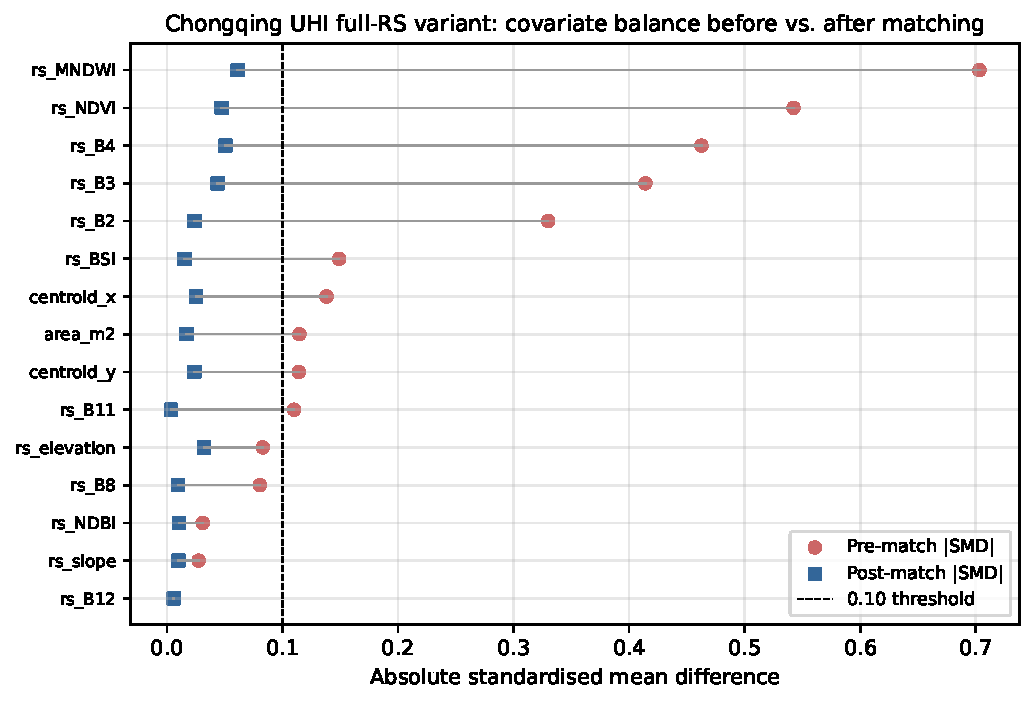
\includegraphics[width=0.86\textwidth]{fig_chongqing_loveplot.pdf}
\caption{Chongqing UHI covariate balance before and after caliper matching (Love plot) for the pre-treatment set. The 0.10 SMD threshold is shown for reference; the maximum post-match SMD is 0.104, a near-threshold miss rather than a strict balance pass.}
\label{fig:loveplot}
\end{figure}

\begin{figure}[htbp]
\centering
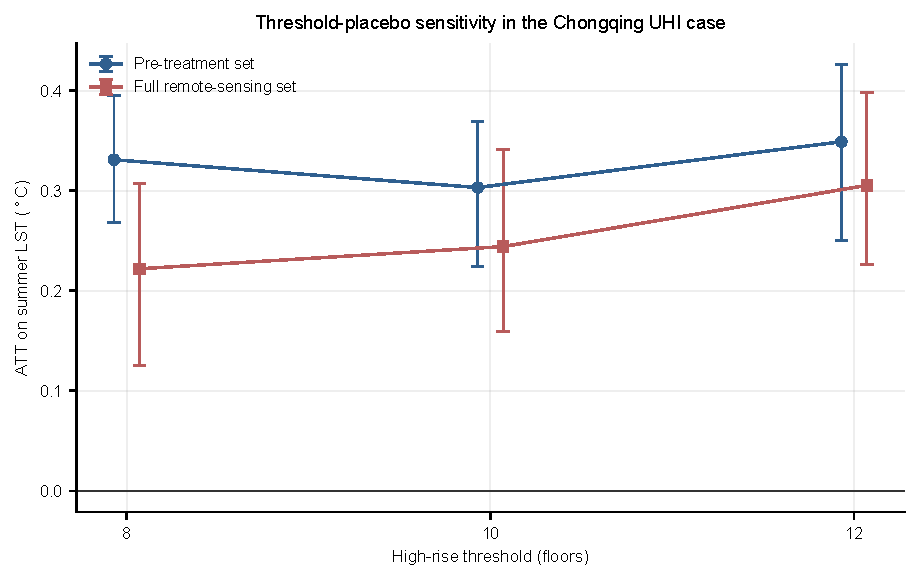
\includegraphics[width=0.82\textwidth]{fig_chongqing_threshold_curve.pdf}
\caption{Chongqing threshold-placebo dose-response. Vertical bars are matching-based 95\% CIs. The monotone increase from 8 to 12 floors is consistent with a dose-response interpretation; all estimates remain small relative to the thermal-retrieval and change-of-support uncertainties that accompany $\sim$1\,km LST extraction.}
\label{fig:threshold}
\end{figure}

\begin{table}[htbp]
\centering
\small
\caption{Chongqing UHI adjustment variants. \emph{pre\_treatment} is preferred because it avoids possible post-treatment Sentinel surfaces but slightly misses strict balance. Balance pass means maximum post-match SMD $<0.10$.}
\label{tab:chongqing}
\setlength{\tabcolsep}{4pt}
\resizebox{\textwidth}{!}{%
\begin{tabular}{lrrrrrl}
\toprule
Variant & ATT ($^\circ$C) & CI lower & CI upper & Max pre SMD & Max post SMD & Role \\
\midrule
Raw difference & 0.238 & 0.163 & 0.307 & -- & -- & unadjusted \\
Coordinates only & 0.267 & 0.178 & 0.346 & 0.138 & 0.080 & pre-treatment \\
Geometry & 0.252 & 0.180 & 0.333 & 0.138 & 0.125 & pre-treatment \\
Terrain & 0.303 & 0.229 & 0.367 & 0.138 & 0.104 & pre-treatment \\
\textbf{Pre-treatment (preferred)} & \textbf{0.303} & \textbf{0.220} & \textbf{0.383} & \textbf{0.138} & \textbf{0.104} & \textbf{confounder-only} \\
Sentinel indices & 0.157 & 0.051 & 0.239 & 0.703 & 0.083 & possible mediator \\
Sentinel bands & 0.121 & 0.034 & 0.210 & 0.463 & 0.051 & possible mediator \\
Full RS context & 0.244 & 0.126 & 0.345 & 0.703 & 0.061 & over-adjusted \\
PCA context & 0.231 & 0.140 & 0.324 & 0.560 & 0.065 & over-adjusted \\
\bottomrule
\end{tabular}
}
\end{table}

The pre-treatment set was chosen for causal role rather than minimum SMD. It uses coordinates, geometry, and terrain, which are more plausibly pre-construction than same-period Sentinel surfaces. Its maximum post-match SMD is 0.104 in the matching-sensitivity audit. The full remote-sensing set improves balance (0.061) and lowers the building-level estimate to 0.244$^\circ$C, but remains an over-adjustment comparison.

Residual Moran's $I$ remained significant for the pre-treatment specification ($I = 0.112$, $p = 0.01$) and full-context set ($I = 0.102$, $p = 0.01$). Under \ruleversion, the default $t_{\mathrm{Moran}}=0.10$ triggers \texttt{material\_residual\_moran}; at 0.15 and 0.20, the residual becomes a significant sub-threshold warning. The claim is therefore an outcome-scale, measured-context association with residual-spatial caution.

Table~\ref{tab:chongqing_estimand_audit} collects reviewer-critical boundaries from the estimand-sensitivity audit: the pixel coefficient is not a building ATT, the near-threshold match is not a strict balance pass, and the residual-Moran grade is not a universal validity class.

\begin{table}[htbp]
\centering
\scriptsize
\caption{Chongqing estimand and sensitivity audit generated from public aggregate outputs. The table records the claim boundary associated with each reviewer-critical diagnostic.}
\label{tab:chongqing_estimand_audit}
\resizebox{\textwidth}{!}{%
\begin{tabular}{L{2.7cm}L{5.4cm}L{4.0cm}L{4.6cm}}
\toprule
Dimension & Quantitative evidence & Claim boundary & Manuscript action \\
\midrule
Outcome-scale estimand & Pixel high-rise-share slope = 0.546$^\circ$C per unit share; building-level matching ATT = 0.303$^\circ$C & Primary result is an outcome-scale association/slope, not a building-level ATT & Rename the primary effect and keep matching as diagnostic \\
Pixel-cluster precision & Naive SE = 0.038; pixel-cluster SE = 0.054; SE inflation = 41.5\% & Building-level precision is overstated unless shared outcome pixels are acknowledged & Report clustered and pixel rows together \\
Balance near miss & Max post-match SMD = 0.104; balance pass = false & The preferred design is near-threshold, not strictly balanced & Keep the match under bounded support \\
Residual threshold margin & Moran's $I = 0.112$; margin above 0.10 = 0.012; grade flips at 0.15 and 0.20 & Grade is threshold-sensitive, while the residual warning remains & Report the threshold-margin audit \\
Process transfer & TPR at $t=0.10$: CAR 0.194, SAR 0.529, kernel 0.994, non-stationary 1.000 & Residual Moran's $I$ is process-dependent, not a universal bias detector & State transfer limits wherever the rule is interpreted \\
Sentinel role boundary & Full-RS max SMD = 0.061 and ATT = 0.244$^\circ$C, but surfaces may be post-treatment & Better balance does not make Sentinel-rich adjustment causally primary & Keep Sentinel as over-adjustment comparison \\
Restricted data & Raw Chongqing inputs are not redistributed; public reconstruction is structural & Exact external reproduction needs approved local inputs & State aggregate-audit scope in Data Availability \\
\bottomrule
\end{tabular}
}
\end{table}

The variable-role audit (Table~\ref{tab:chongqing_roles}) separates admissibility from balance. Coordinates and terrain are low-risk, geometry is a medium-risk morphology proxy, and Sentinel-derived features are ambiguous proxies or possible mediators. The preferred set trades slightly weaker balance for a more defensible causal role.

\begin{table}[htbp]
\centering
\scriptsize
\caption{Chongqing variable-role audit for candidate spatial-context sources. Risk describes possible post-treatment or mediator contamination, not statistical balance.}
\label{tab:chongqing_roles}
\resizebox{\textwidth}{!}{%
\begin{tabular}{L{2.5cm}L{3.2cm}L{2.0cm}L{2.5cm}rrL{1.7cm}}
\toprule
Context group & Causal role & Risk & Variant & ATT ($^\circ$C) & Max post SMD & Balance pass \\
\midrule
Coordinates & Spatial proxy confounder & Low & coordinates only & 0.267 & 0.080 & Yes \\
Building geometry & Proxy confounder or pre-treatment morphology & Medium & geometry & 0.252 & 0.125 & No \\
Terrain & Pre-treatment confounder & Low & terrain & 0.303 & 0.104 & No \\
\textbf{Pre-treatment (preferred)} & Confounder-only adjustment set & Low & pre\_treatment & 0.303 & 0.104 & No \\
Sentinel indices & Ambiguous proxy or mediator & High & sentinel indices & 0.157 & 0.083 & Yes \\
Sentinel bands & Ambiguous proxy or mediator & Medium & sentinel bands & 0.121 & 0.051 & Yes \\
Full RS context & Over-adjusted (possible mediators) & Medium & full RS context & 0.244 & 0.061 & Yes \\
\bottomrule
\end{tabular}
}
\end{table}

\begin{figure}[htbp]
\centering
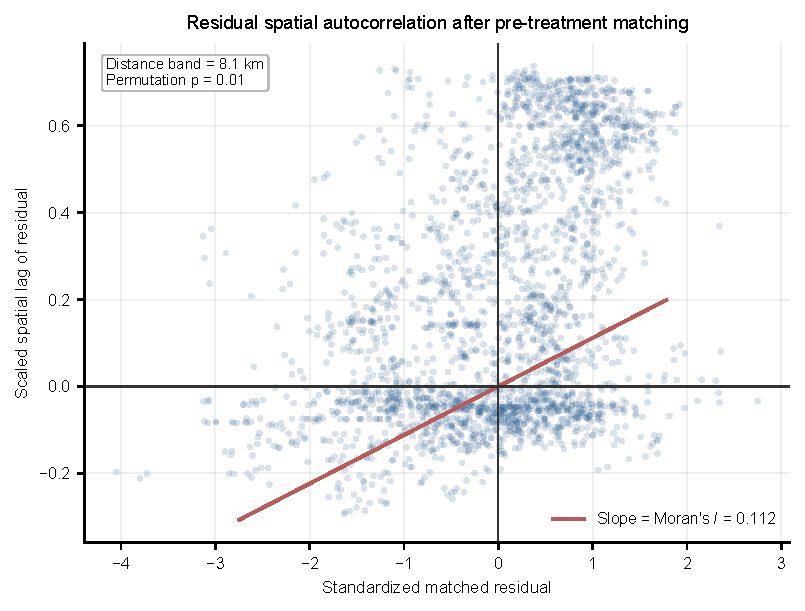
\includegraphics[width=0.66\textwidth]{fig_chongqing_residual_moran.pdf}
\caption{Empirical Moran scatter for the Chongqing matched pre-treatment residual (standardised residual on the $x$-axis, its spatial lag on the $y$-axis). The slope is the empirical Moran's $I = 0.112$, statistically significant under 99 permutations ($p=0.01$); under the default 0.10 rule it triggers a material residual-spatial caution, while under a high-specificity 0.20 sensitivity threshold it would be recorded as significant-below-material.}
\label{fig:residual}
\end{figure}

\subsection{County ArcGIS SCI Plus workflow comparison}

The county run tests whether SCCA can reproduce the documented ArcGIS Causal Inference algorithm and show how causal-risk diagnostics change interpretation. The target is the continuous-exposure ArcGIS mode: regression propensity scores, matching balance over exposure bins and propensity-score scale, plug-in weighted-kernel ERF smoothing, and target-response lookup \citep{esri2026causalworks,wu2022matching,fan1996local}. The exposure is county social association, the outcome is average age at death, and the unit is the contiguous U.S.\ county. The runner exports field-level provenance and embeds the same summary in the machine-readable SCI Plus report; unemployment is marked as lineage-only because the metadata names the joined table and field but not a separate external producer citation.

After 1\%--99\% exposure trimming, 3{,}044 of 3{,}108 counties remained, matching the local ArcGIS Pro 3.7 arcpy run. The open documented-mode runner used the same selected ArcGIS parameters (25 exposure bins, propensity/exposure scale 0.8) and a plug-in bandwidth of 2.439, compared with 2.4415 from arcpy. Its mean absolute weighted confounder correlation was 0.072, below the 0.10 balance threshold (arcpy: 0.0559). The 200-point ERF curve was nearly identical to the native arcpy ERF (MAE = 0.015 years; RMSE = 0.044). Thus, for this documented mode, SCCA can replace the ArcGIS Causal Inference algorithmic task in open, scriptable workflows. This is not a bit-for-bit claim for untested ArcGIS modes such as gradient boosting, weighting, cross-validated bandwidths, or bootstrap intervals.

The target-response audit still records a boundary: 70 years lies below the trimmed ERF response range (73.91--81.87), so the solver returns the nearest ERF point rather than a supported exposure attaining 70. A geometry-enabled notebook supplied spatial diagnostics: adjusted OLS was 0.181, spatial-lag sensitivity was 0.145, residual Moran's $I$ remained 0.313 ($p = 0.010$), and neighbor exposure was significant ($p < 0.001$). The rule table therefore assigns bounded support.

\subsection{Synthetic positive control (discrimination test)}
\label{sec:core_control}

Because the empirical cases are bounded, we include a synthetic positive control. It generates a clean DGP with $n=3{,}000$, measured confounders, excellent overlap, and no latent spatial process. The control recovers the true effect (ATT $=0.505$ vs.\ true $0.5$; relative bias $<1\%$), passes balance, has non-significant residual Moran's $I$ and neighbor exposure, and receives \emph{core support}. Thus bounded empirical grades reflect diagnostics, not a rule engine that always downgrades.

\subsection{Baseline-to-SCCA comparison}

The reproduction package stores the direct comparisons. In Chongqing, estimates moved from 0.238$^\circ$C raw to 0.303$^\circ$C pre-treatment and 0.244$^\circ$C over-adjusted. In the county case, the spatial layer reduced the coefficient from 0.181 to 0.145 and downgraded evidence because residual Moran's $I$ and neighbor exposure remained significant.

\subsection{Threshold calibration for the residual-Moran rule}
\label{sec:thresholdcalibration}

We calibrated the material residual-Moran threshold $t_{\mathrm{Moran}}$ across SAR, CAR, distance-kernel, and non-stationary latent processes. The script sweeps $\rho \in \{0.2, 0.5, 0.8\}$, $n \in \{400, 900, 1600\}$ and $\sigma_u \in \{0, 0.5, 1, 2\}$ for 20 replicates per cell and family, producing 2{,}880 SCCA fits with known ATT = 0.5. For each fit it records material bias (relative bias $> 25\%$) and threshold firing; outputs are included in the reproduction package.

Table~\ref{tab:moran_roc} reports the pooled trade-off and Figure~\ref{fig:rocs} the ROC. Pooling across families, the Youden's $J$ optimum sits at $t = 0.05$ (TPR $= 0.79$, FPR $= 0.03$), while $t=0.10$ keeps a low false-positive rate (0.02) and recovers 68\% of materially biased fits. The 2026-06-30 rule set uses $t_{\mathrm{Moran}}=0.10$ as the default conservative threshold and treats 0.20 as a high-specificity sensitivity threshold.

The trade-off is \emph{family-dependent} (Table~\ref{tab:moran_family}). Kernel and non-stationary fields produce large biased residual Moran's $I$ (means 0.32 and 0.40), with TPR $\geq 0.99$ even at $t=0.20$. CAR fields leave small residual Moran's $I$ (mean 0.04), so $t=0.10$ recovers only 19\% of biased CAR fits and $t=0.20$ essentially none. SAR is intermediate (TPR 0.53 at $t=0.10$). The rule is therefore a useful but process-dependent warning boundary, not a universal detector.

\begin{table}[htbp]
\centering
\small
\caption{Pooled calibration of the SCCA residual-Moran downgrade rule across four spatial-process families (2{,}880 fits). Positive class: relative bias $>$ 25\%. Predictor: $|I_{\mathrm{residual}}| \geq t$ AND permutation $p \leq 0.05$.}
\label{tab:moran_roc}
\setlength{\tabcolsep}{4pt}
\begin{tabular}{cccccL{4.2cm}}
\toprule
Threshold $t$ & TPR & FPR & Precision & Youden's $J$ & Verdict \\
\midrule
0.05 & 0.79 & 0.030 & 0.99 & 0.762 & pooled Youden optimum \\
0.10 & 0.68 & 0.023 & 0.99 & 0.657 & manuscript default; flags Chongqing \\
0.15 & 0.59 & 0.019 & 0.99 & 0.573 & \\
0.20 & 0.57 & 0.018 & 0.99 & 0.556 & high-specificity sensitivity \\
0.25 & 0.55 & 0.014 & 0.99 & 0.534 & \\
0.30 & 0.50 & 0.008 & 0.99 & 0.494 & too lenient \\
\bottomrule
\end{tabular}
\end{table}

\begin{table}[htbp]
\centering
\footnotesize
\caption{Per-family behaviour of the residual-Moran rule. Mean residual Moran's $I$ is averaged over all cells of that family; TPR is at the manuscript default $t=0.10$. The rule is strong for kernel/non-stationary processes but weak for CAR, where the same relative bias leaves little simple-contiguity autocorrelation in the residual.}
\label{tab:moran_family}
\setlength{\tabcolsep}{4pt}
\begin{tabular}{@{}L{3.35cm}rrrr@{}}
\toprule
Latent-process family & \shortstack{Mean\\residual $I$} & \shortstack{TPR\\@ 0.10} & \shortstack{TPR\\@ 0.20} & \shortstack{Family Youden-\\optimal $t$} \\
\midrule
CAR (conditional AR) & 0.04 & 0.19 & 0.00 & 0.05 \\
SAR (simultaneous AR) & 0.10 & 0.53 & 0.30 & 0.05 \\
Exponential kernel & 0.32 & 0.99 & 0.99 & 0.20 \\
Non-stationary & 0.40 & 1.00 & 1.00 & 0.05 \\
\bottomrule
\end{tabular}
\end{table}

\begin{figure}[htbp]
\centering
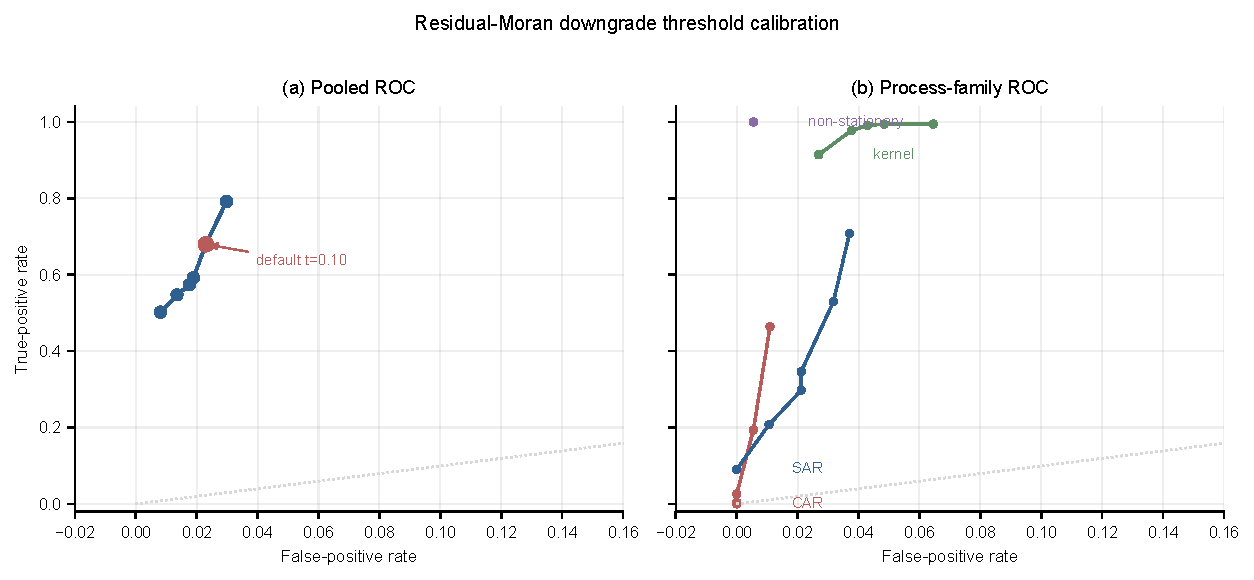
\includegraphics[width=0.92\textwidth]{fig_threshold_calibration_roc.pdf}
\caption{Threshold calibration for the SCCA residual-Moran downgrade rule. (a) Pooled ROC across candidate material thresholds. (b) Per-family ROC (process-dependent power): the 0.10 threshold, calibrated on a pooled design, exhibits strong external validity for kernel and non-stationary families (TPR $\approx$ 1.0) but limited power for CAR structures (TPR = 0.19), showing that the rule's discriminative ability depends on the unknown latent spatial process.}
\label{fig:rocs}
\end{figure}

\subsection{Grade-rule sensitivity for the two case studies}
\label{sec:chongqing_threshold_check}

The county grade is stable, but the Chongqing grade is boundary-dependent. Varying only the residual-Moran threshold, Chongqing changes from bounded support at 0.10 to a significant sub-threshold warning at 0.15 and 0.20. County remains bounded because residual Moran's $I=0.313$ and neighboring exposure stay significant.

\begin{table}[htbp]
\centering
\scriptsize
\caption{Residual-spatial threshold sensitivity generated by the evidence-synthesis script. The exercise varies only the material residual Moran warning threshold and leaves all other downgrade rules unchanged.}
\label{tab:grade_threshold_sensitivity}
\resizebox{\textwidth}{!}{%
\begin{tabular}{L{3.6cm}rrL{1.9cm}L{4.0cm}L{4.1cm}}
\toprule
Case & Residual Moran's $I$ & Threshold & Grade & Residual status & Grade rules or flags \\
\midrule
Chongqing pre-treatment & 0.112 & 0.10 & Bounded & material significant & \texttt{material\_residual\_moran} \\
Chongqing pre-treatment & 0.112 & 0.15 & Core & significant below material threshold & non-downgrade residual warning \\
Chongqing pre-treatment & 0.112 & 0.20 & Core & significant below material threshold & non-downgrade residual warning \\
County spatial notebook & 0.313 & 0.10 & Bounded & material significant & \texttt{material\_residual\_moran}; \texttt{significant\_neighbor\_exposure} \\
County spatial notebook & 0.313 & 0.15 & Bounded & material significant & \texttt{material\_residual\_moran}; \texttt{significant\_neighbor\_exposure} \\
County spatial notebook & 0.313 & 0.20 & Bounded & material significant & \texttt{material\_residual\_moran}; \texttt{significant\_neighbor\_exposure} \\
\bottomrule
\end{tabular}
}
\end{table}

County response-shape checks also varied the social-capital knot. A knot at 13 gave an after-knot slope increase of 0.104 years per unit (HC3 $p=0.00075$; AIC improvement = 17.46), but other knots changed strength. This supports the county run as operational sensitivity, not independent causal evidence.

\subsection{GIS and notebook outputs}

The county notebook also tested SCCA as an operational GIS workflow. The shared core wrote joined tables, GeoPackage, GeoJSON, Shapefile, maps, and QGIS \texttt{.qml} styles from the same \texttt{AnalysisRequest}. These outputs do not strengthen identification; they make assumptions and spatial cautions visible in GIS environments.

% ============================================================================
\section{Discussion}
\label{sec:discussion}
% ============================================================================

\subsection{What SCCA solves}

SCCA addresses a practical gap: spatial variables are often added without showing whether they improved adjustment, and spatial residuals are treated as model diagnostics rather than claim boundaries. SCCA makes the adjustment set inspectable through context variants, balance, support, spatial checks, and evidence grades.

The Chongqing case shows why this record matters. Because the outcome is measured on MODIS pixels, the defensible quantity is the outcome-scale high-rise-share slope, not the building match. The paper reports that slope with diagnostic matching, variable-role and estimand audits, residual Moran's $I = 0.112$ ($p = 0.01$), and a bounded grade. The best-balanced Sentinel set attenuates the building estimate from 0.303 to 0.244$^\circ$C, but may be post-treatment.

The county notebook shows the same logic for GIS use: ArcGIS SCI-style trim, ERF, and target outputs remain visible while target-support, residual-autocorrelation, and neighboring-exposure diagnostics bound the claim.

\subsection{Practical value for GIS workflows}

SCCA converts a causal analysis into an inspectable spatial evidence package. The ArcGIS toolbox, QGIS provider, notebook workflow, and command-line interface share one request object and manifest, reducing divergence across notebooks, desktop joins, and publication tables.

The county comparison is concrete: the workbook-level SCI Plus run reproduced the native arcpy continuous-exposure ERF with MAE = 0.015 years while exposing target-support warnings, field-level provenance, role/scale risk fields, a replacement-assessment field, and explicit bias-bound status; the geometry-enabled notebook added spatial diagnostics. This is reproducibility for the tested ArcGIS Causal Inference mode and auditability, not independent causal validation. The central novelty is the audit layer that turns an ERF estimate into a provenance-linked, support-aware, spatial-risk-classified evidence object. Untested ArcGIS modes require separate parity tests.

GIS outputs are audit objects, not causal evidence by themselves.

\subsection{How SCCA can be extended}

The workflow can be strengthened by adding formal sensitivity analysis for unmeasured spatial confounding, making variable-role declarations mandatory, using spatial cross-fitting for high-dimensional nuisance models, and separating SLX-style diagnostics from formal interference estimands \citep{chernozhukov2018dml,forastiere2021interference,papadogeorgou2022causal}. Scale remains central: buffer radius, aggregation, and neighborhood definitions should be part of the adjustment design. The new aggregate Chongqing audit is still not a substitute for latent-confounder sensitivity analysis on restricted building-level data.

\subsection{What SCCA does not solve}

SCCA does not make observational spatial data equivalent to randomised experiments. It cannot adjust for absent confounders or automatically solve interference. SLX-style summaries are sensitivity outputs, not identified network-interference estimands \citep{forastiere2021interference,papadogeorgou2022causal}. In Chongqing, high-rise heat may affect adjacent pixels, so SUTVA is unlikely to hold exactly. The building-level ATT can conflate own contrast with spillover; the outcome-scale slope reduces support mismatch but does not identify spillover. Future work should use spillover-robust methods \citep{aronow2017interference} or explicit interference models when neighborhood contamination is the question.

SCCA also does not remove MAUP or treatment-outcome scale mismatch \citep{openshaw1984maup,fotheringham1991modifiable}. The pixel-level slope in Table~\ref{tab:cos} assumes the data-generating process is meaningful at pixel scale; if reality is finer, that estimand remains mis-specified. Context variables are audited by variants, missingness handling remains conservative, and only the residual-Moran rule is calibrated here.

The Chongqing interpretation is therefore bounded by five visible limits: residual spatial structure, building-to-pixel support mismatch, possible post-treatment Sentinel ambiguity, residual-Moran threshold sensitivity, and restricted raw inputs. These are properties of the data that SCCA makes visible.

% ============================================================================
\section{Conclusions}
\label{sec:conclusions}
% ============================================================================

We presented Spatial Context Causal Adjustment, an open diagnostic workflow for geographic observational causal studies. SCCA evaluates spatial-context variants through support, balance, robustness, spatial diagnostics, variable-role audits, and evidence-grade rules. A 2{,}880-fit calibration showed that the residual-Moran downgrade is useful but process-dependent; the synthetic, Chongqing, and county checks distinguished useful estimates from bounded or fragile designs.

The main empirical result is deliberately bounded. In Chongqing, the outcome-scale pixel model estimated a positive high-rise-share slope for summer LST (0.546$^\circ$C per unit share, 95\% CI [0.359, 0.734]); building-level matching (0.303$^\circ$C) is diagnostic because treatment is finer than MODIS support. The preferred set slightly missed balance, residual Moran's $I = 0.112$ crossed the default rule, and Sentinel surfaces may be post-treatment. SCCA makes assumptions, diagnostics, and claim boundaries visible in GIS-facing workflows.


% ============================================================================
\section*{Declaration of Competing Interest}
% ============================================================================

The author declares no competing financial interests or personal relationships.

\section*{Acknowledgements}
% ============================================================================

The author thanks colleagues for early discussions of the SCCA workflow.

\section*{Funding}
% ============================================================================

No external funding was used.

\section*{AI Use Statement}
% ============================================================================

The author used AI-assisted tools for language editing, code drafting, consistency checks, and pre-submission audit. The author checked all analyses, outputs, interpretations, and final text.

\section*{Data and Code Availability}
% ============================================================================

For peer review, code, manuscript source, generators, tables, figures, diagnostics, and redistributable public/example data are in the anonymized repository: \url{https://anonymous.4open.science/r/spatial-causal-inference-FDFE}. It supports exact synthetic and county/example reruns and structural Chongqing reruns from approved restricted inputs. Raw Chongqing geospatial inputs and the building-level UHI sample are not redistributed because they include precise geometries or coordinates, floor attributes, and derived environmental variables. The repository instead provides aggregate balance, diagnostic, and matching-sensitivity artifacts and does not claim full public reconstruction of the restricted Chongqing result. After peer review, it can be linked to the public archival repository if required.

The county social-capital case uses third-party Esri training/demo data credited in metadata to Esri, the U.S. Census Bureau, NOAA/NOS/NGS, CDC WONDER/NCHS, and 2019 County Health Rankings/Living Atlas. Field-level provenance is in the SCI Plus \texttt{data\_provenance} block; one unemployment covariate remains lineage-only. Use follows the Esri Master License and is restricted to training, demonstration, and educational purposes. Evidence synthesis, rule tables, audits, method comparison, and public summaries are included.



\begin{thebibliography}{99}

\bibitem[Abadie and Imbens, 2006]{abadie2006matchingse}
Abadie, A. and Imbens, G.W., 2006. Large sample properties of matching estimators for average treatment effects. Econometrica 74(1), 235--267.

\bibitem[Angrist and Pischke, 2009]{angrist2009mostly}
Angrist, J.D. and Pischke, J.S., 2009. Mostly Harmless Econometrics: An Empiricist's Companion. Princeton University Press.

\bibitem[Anselin, 1988]{anselin1988spatial}
Anselin, L., 1988. Spatial Econometrics: Methods and Models. Kluwer Academic Publishers.

\bibitem[Anselin and Rey, 2014]{anselin2014modern}
Anselin, L. and Rey, S.J., 2014. Modern Spatial Econometrics in Practice: A Guide to GeoDa, GeoDaSpace and PySAL. GeoDa Press.

\bibitem[Aronow and Samii, 2017]{aronow2017interference}
Aronow, P.M. and Samii, C., 2017. Estimating average causal effects under general interference, with application to a social network experiment. Annals of Applied Statistics 11(4), 1912--1947.

\bibitem[Athey and Imbens, 2019]{athey2019estimating}
Athey, S. and Imbens, G.W., 2019. Machine Learning Methods That Economists Should Know About. Annual Review of Economics 11, 685--725.

\bibitem[Austin, 2009]{austin2009smd}
Austin, P.C., 2009. Balance diagnostics for comparing the distribution of baseline covariates between treatment groups in propensity-score matched samples. Statistics in Medicine 28(25), 3083--3107.

\bibitem[Brunsdon, 2016]{brunsdon2016quantitative}
Brunsdon, C., 2016. Quantitative methods I. Progress in Human Geography 40(5), 687--696. doi:10.1177/0309132515599625.

\bibitem[Chernozhukov et~al., 2018]{chernozhukov2018dml}
Chernozhukov, V., Chetverikov, D., Demirer, M., Duflo, E., Hansen, C., Newey, W. and Robins, J., 2018. Double/debiased machine learning for treatment and structural parameters. Econometrics Journal 21(1), C1--C68.

\bibitem[Dupont et~al., 2022]{dupont2022spatial+}
Dupont, E., Wood, S.N. and Augustin, N.H., 2022. Spatial+: a novel approach to spatial confounding. Biometrics 78(4), 1279--1290.

\bibitem[Forastiere et~al., 2021]{forastiere2021interference}
Forastiere, L., Airoldi, E.M. and Mealli, F., 2021. Identification and estimation of treatment and interference effects in observational studies on networks. Journal of the American Statistical Association 116(534), 901--918.

\bibitem[Fotheringham and Wong, 1991]{fotheringham1991modifiable}
Fotheringham, A.S. and Wong, D.W.S., 1991. The modifiable areal unit problem in multivariate statistical analysis. Environment and Planning A 23(7), 1025--1044.

\bibitem[Giffin et~al., 2023]{giffin2023gpsinterference}
Giffin, A., Reich, B.J., Yang, S. and Rappold, A.G., 2023. Generalized Propensity Score Approach to Causal Inference with Spatial Interference. Biometrics 79(3), 2220--2231. doi:10.1111/biom.13745.

\bibitem[Esri, 2026]{esri2026causalworks}
Esri, 2026. How Causal Inference Analysis works. ArcGIS Pro documentation. Available at: https://pro.arcgis.com/en/pro-app/latest/tool-reference/spatial-statistics/how-causal-inference-analysis-works.htm (accessed 4 July 2026).

\bibitem[Fan, 1996]{fan1996local}
Fan, J. and Gijbels, I., 1996. Local Polynomial Modelling and Its Applications. Chapman \& Hall.
\bibitem[Gilbert et~al., 2021]{gilbert2021spatialconfounding}
Gilbert, B., Datta, A., Casey, J.A. and Ogburn, E.L., 2021. A causal inference framework for spatial confounding. arXiv:2112.14946.

\bibitem[Hern\'an and Robins, 2020]{hernan2020whatif}
Hern\'an, M.A. and Robins, J.M., 2020. Causal Inference: What If. Chapman \& Hall/CRC.

\bibitem[Hirano and Imbens, 2004]{hirano2004gps}
Hirano, K. and Imbens, G.W., 2004. The propensity score with continuous treatments. In: Gelman, A. and Meng, X.-L., eds. Applied Bayesian Modeling and Causal Inference from Incomplete-Data Perspectives. Wiley, 73--84.

\bibitem[Hodges and Reich, 2010]{hodges2010adding}
Hodges, J.S. and Reich, B.J., 2010. Adding spatially-correlated errors can mess up the fixed effect you love. The American Statistician 64(4), 325--334.

\bibitem[Imbens and Rubin, 2015]{imbens2015causal}
Imbens, G.W. and Rubin, D.B., 2015. Causal Inference for Statistics, Social, and Biomedical Sciences. Cambridge University Press.

\bibitem[Khan and Calder, 2022]{khan2022restricted}
Khan, K. and Calder, C.A., 2022. Restricted Spatial Regression Methods: Implications for Inference. Journal of the American Statistical Association 117(537), 482--494. doi:10.1080/01621459.2020.1788949.

\bibitem[Konkol and Kray, 2019]{konkol2019computational}
Konkol, M. and Kray, C., 2019. In-depth examination of spatiotemporal figures in open reproducible research. Cartography and Geographic Information Science 46(5), 412--427. doi:10.1080/15230406.2018.1512421.

\bibitem[LeSage and Pace, 2009]{lesage2009introduction}
LeSage, J.P. and Pace, R.K., 2009. Introduction to Spatial Econometrics. CRC Press.

\bibitem[Manley et~al., 2006]{manley2006maup}
Manley, D., Flowerdew, R. and Steel, D., 2006. Scales, levels and processes: studying spatial patterns of British census variables. Computers, Environment and Urban Systems 30(2), 143--160.

\bibitem[N\"ust and Pebesma, 2021]{nuest2021reproducible}
N\"ust, D. and Pebesma, E., 2021. Practical reproducibility in geography and geosciences. Annals of the American Association of Geographers 111(5), 1300--1310.

\bibitem[Openshaw, 1984]{openshaw1984maup}
Openshaw, S., 1984. The Modifiable Areal Unit Problem. CATMOG 38, Geo Books, Norwich.

\bibitem[Paciorek, 2010]{paciorek2010importance}
Paciorek, C.J., 2010. The importance of scale for spatial-confounding bias and precision of spatial regression estimators. Statistical Science 25(1), 107--125.

\bibitem[Papadogeorgou et~al., 2022]{papadogeorgou2022causal}
Papadogeorgou, G., Imai, K., Lyall, J. and Li, F., 2022. Causal inference with spatio-temporal data: Estimating the effects of airstrikes on insurgent violence in Iraq. Journal of the Royal Statistical Society Series B 84(5), 1969--1999.

\bibitem[Pearl, 2009]{pearl2009causality}
Pearl, J., 2009. Causality: Models, Reasoning, and Inference. 2nd ed. Cambridge University Press.

\bibitem[Reich et~al., 2021]{reich2021review}
Reich, B.J., Yang, S., Guan, Y., Giffin, A.B., Miller, M.J. and Rappold, A.G., 2021. A Review of Spatial Causal Inference Methods for Environmental and Epidemiological Applications. International Statistical Review 89(3), 605--634. doi:10.1111/insr.12452.

\bibitem[Rosenbaum and Rubin, 1983]{rosenbaum1983central}
Rosenbaum, P.R. and Rubin, D.B., 1983. The central role of the propensity score in observational studies for causal effects. Biometrika 70(1), 41--55.

\bibitem[Schnell and Papadogeorgou, 2020]{schnell2020mitigating}
Schnell, P.M. and Papadogeorgou, G., 2020. Mitigating unobserved spatial confounding when estimating the effect of supermarket access on cardiovascular disease deaths. Annals of Applied Statistics 14(4), 2069--2095.

\bibitem[Stuart, 2010]{stuart2010matching}
Stuart, E.A., 2010. Matching Methods for Causal Inference: A Review and a Look Forward. Statistical Science 25(1), 1--21.

\bibitem[Tec et~al., 2023]{tec2023spatialdml}
Tec, M., Scott, J.G. and Zigler, C.M., 2023. Weather2vec: Representation Learning for Causal Inference with Non-local Confounding in Air Pollution and Climate Studies. Proceedings of the AAAI Conference on Artificial Intelligence 37(12), 14504--14513. doi:10.1609/aaai.v37i12.26696.

\bibitem[VanderWeele, 2015]{vanderweele2015explanation}
VanderWeele, T.J., 2015. Explanation in Causal Inference: Methods for Mediation and Interaction. Oxford University Press.

\bibitem[Verbitsky-Savitz and Raudenbush, 2012]{verbitskysavitz2012}
Verbitsky-Savitz, N. and Raudenbush, S.W., 2012. Causal inference under interference in spatial settings: A case study evaluating community policing program in Chicago. Epidemiologic Methods 1(1), 107--130.

\bibitem[Wu et~al., 2024]{wu2022matching}
Wu, X., Mealli, F., Kioumourtzoglou, M.-A., Dominici, F. and Braun, D., 2024. Matching on Generalized Propensity Scores with Continuous Exposures. Journal of the American Statistical Association 119(545), 757--772. doi:10.1080/01621459.2022.2144737.
\bibitem[Zhao et~al., 2020]{zhao2020nonbinary}
Zhao, S., van Dyk, D.A. and Imai, K., 2020. Propensity score-based methods for causal inference in observational studies with non-binary treatments. Statistical Methods in Medical Research 29(3), 709--727. doi:10.1177/0962280219888745.

\end{thebibliography}

\end{document}
